\chapter{Технологическая часть}

\section{Средства реализации}

Для программной реализации шифровальной машины был выбран язык Rust. В данном языке есть все требующиеся инструменты для данной лабораторной работы.

\section{Реализация алгоритма}

В листингах~\ref{lst:keygen}~---~\ref{lst:edcrypt} представлена реализация алгоритма DES.

\begin{center}
\captionsetup{justification=raggedright,singlelinecheck=off}
\begin{lstlisting}[label=lst:keygen,caption=Генерация ключа]
mod hex {
    pub fn encode(b: &[u8]) -> String {
        let mut s = String::with_capacity(b.len() * 2);
        for &byte in b {
            s.push(hex_char(byte >> 4));
            s.push(hex_char(byte & 0xF));
        }
        s
    }
}

pub fn genkey_file(keyfile: &Path) -> Result<(), String> {
    let mut key = [0u8; 8];
    OsRng.fill_bytes(&mut key);

    let hex = hex::encode(&key);

    let mut f = File::create(keyfile).map_err(|e| format!("Failed create keyfile: {}", e))?;
    f.write_all(hex.as_bytes())
        .map_err(|e| format!("Failed write keyfile: {}", e))?;

    Ok(())
}
\end{lstlisting}
\end{center}

\begin{center}
\captionsetup{justification=raggedright,singlelinecheck=off}
\begin{lstlisting}[label=lst:edcrypt,caption=Шифрование/расшифровка алгоритмом RSA]
fn f_func(r: &[u8], k: &[u8]) -> Vec<u8> {
    let r_exp = bits::permute(r, &E);
    let x = bits::xor_bits(&r_exp, k);
    let s_out = sbox_substitute(&x);
    bits::permute(&s_out, &P)
}

fn des_block(block: &[u8; 8], subkeys: &Vec<Vec<u8>>, encrypt: bool) -> [u8; 8] {
    let bits = bits::bytes_to_bitvec(block);
    let ip = bits::permute(&bits, &IP);

    let mut l = ip[..32].to_vec();
    let mut r = ip[32..].to_vec();

    let keys_iter: Box<dyn Iterator<Item = &Vec<u8>>> = if encrypt {
        Box::new(subkeys.iter())
    } else {
        Box::new(subkeys.iter().rev())
    };

    for k in keys_iter {
        let new_l = r.clone();
        let f_out = f_function(&r, k);
        let new_r = bits::xor_bits(&l, &f_out);
        l = new_l;
        r = new_r;
    }

    let preout: Vec<u8> = r.into_iter().chain(l.into_iter()).collect();
    let final_bits = bits::permute(&preout, &FP);
    let out_bytes = bits::bitvec_to_bytes(&final_bits);

    let mut arr = [0u8; 8];
    arr.copy_from_slice(&out_bytes[..8]);
    arr
}

fn pkcs5_pad(data: &[u8]) -> Vec<u8> {
    let pad_len = 8 - (data.len() % 8);
    let mut out = data.to_vec();

    out.extend(std::iter::repeat(pad_len as u8).take(pad_len));
    out
}

fn pkcs5_unpad(data: &[u8]) -> Result<Vec<u8>, String> {
    if data.len() == 0 || data.len() % 8 != 0 {
        return Err("Invalid padded data length".to_string());
    }

    let pad_len = *data.last().unwrap() as usize;
    if pad_len < 1 || pad_len > 8 {
        return Err("Invalid padding byte".to_string());
    }

    let end = data.len();
    for &b in &data[end - pad_len..] {
        if b as usize != pad_len {
            return Err("Invalid padding contents".to_string());
        }
    }

    Ok(data[..end - pad_len].to_vec())
}

pub fn encrypt_file(keyfile: &Path, infile: &Path, outfile: &Path) -> Result<(), String> {
    let key = load_key(keyfile)?;
    let subkeys = generate_subkeys(&key);

    let plaintext = fs::read(infile).map_err(|e| format!("Failed read infile: {}", e))?;
    let padded = pkcs5_pad(&plaintext);

    let mut out = Vec::with_capacity(padded.len());
    for chunk in padded.chunks(8) {
        let mut arr = [0u8; 8];
        arr.copy_from_slice(chunk);
        
        let enc = des_block(&arr, &subkeys, true);
        out.extend_from_slice(&enc);
    }

    let mut f = File::create(outfile).map_err(|e| format!("Failed create outfile: {}", e))?;
    f.write_all(&out)
        .map_err(|e| format!("Failed write outfile: {}", e))?;

    Ok(())
}

pub fn decrypt_file(keyfile: &Path, infile: &Path, outfile: &Path) -> Result<(), String> {
    let key = load_key(keyfile)?;
    let subkeys = generate_subkeys(&key);

    let ciphertext = fs::read(infile).map_err(|e| format!("Failed read infile: {}", e))?;
    if ciphertext.len() % 8 != 0 {
        return Err("Ciphertext length not multiple of 8".to_string());
    }

    let mut out = Vec::with_capacity(ciphertext.len());
    for chunk in ciphertext.chunks(8) {
        let mut arr = [0u8; 8];
        arr.copy_from_slice(chunk);

        let dec = des_block(&arr, &subkeys, false);
        out.extend_from_slice(&dec);
    }

    let unp = pkcs5_unpad(&out).map_err(|e| format!("Unpad error: {}", e))?;

    let mut f = File::create(outfile).map_err(|e| format!("Failed create outfile: {}", e))?;
    f.write_all(&unp)
        .map_err(|e| format!("Failed write outfile: {}", e))?;

    Ok(())
}
\end{lstlisting}
\end{center}

\clearpage

\section{Пример работы программы}

На рисунке~\ref{fig:tex} представлен пример работы программы на текстовом фале.

\begin{figure}[h]
    \centering
    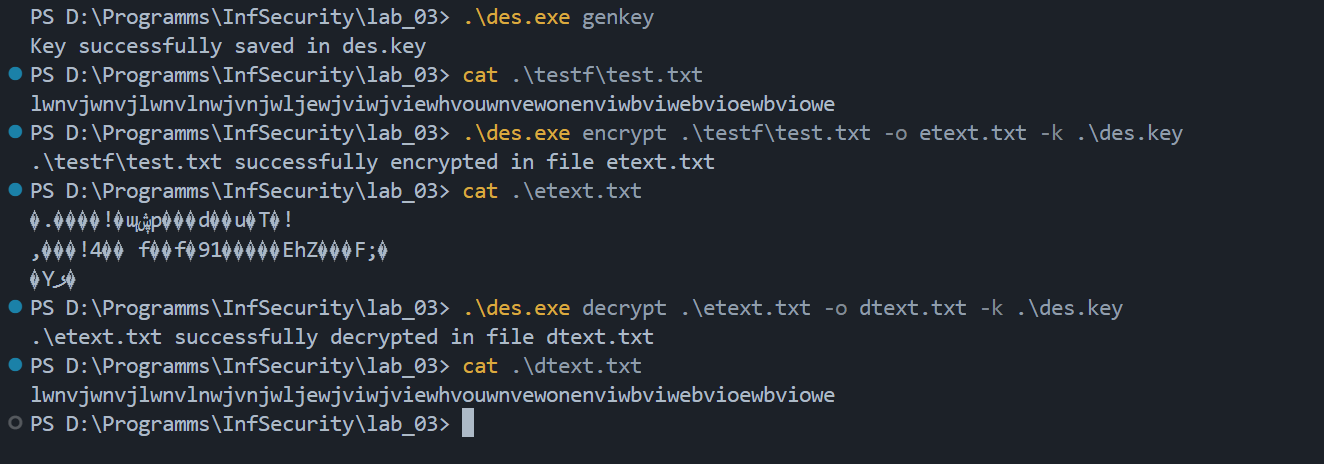
\includegraphics[width=1\linewidth]{images/tex.png}
    \caption{Пример работы программы на текстовом файле}
    \label{fig:tex}
\end{figure}

На рисунках~\ref{fig:zex}~---~\ref{fig:zd} представлен пример работы программы на zip-фале.

\begin{figure}[h]
    \centering
    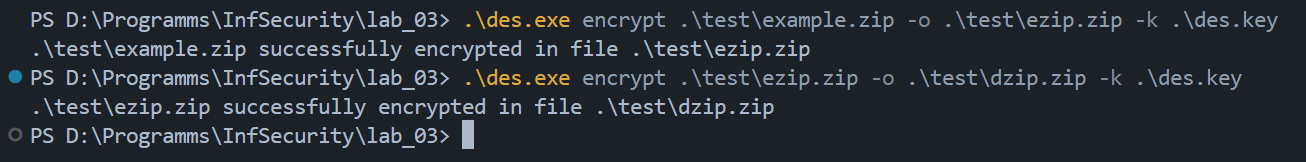
\includegraphics[width=0.9\linewidth]{images/zex.png}
    \caption{Шифрация/дешифрация zip-файла}
    \label{fig:zex}
\end{figure}

\begin{figure}[h]
    \centering
    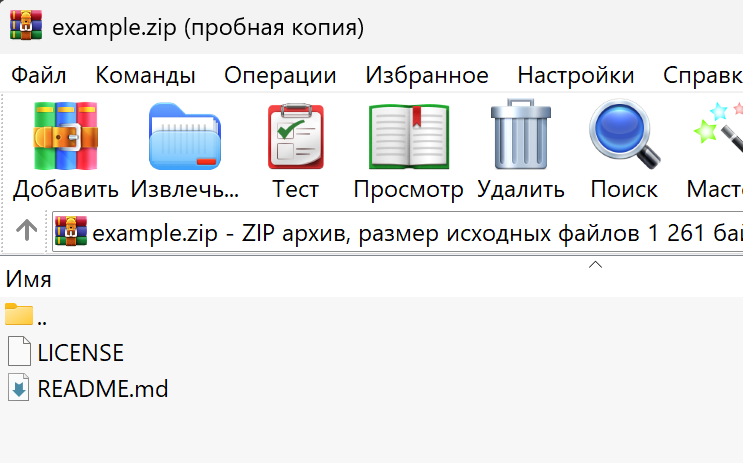
\includegraphics[width=0.6\linewidth]{images/fzip.png}
    \caption{Пример zip-файла}
    \label{fig:z1}
\end{figure}

\begin{figure}[h]
    \centering
    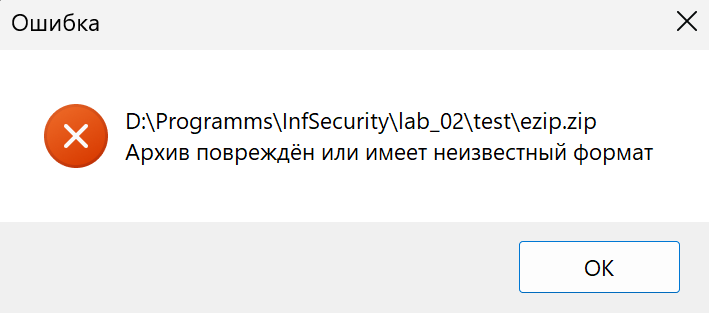
\includegraphics[width=0.6\linewidth]{images/ezip.png}
    \caption{Зашифрованный zip-файл}
    \label{fig:ze}
\end{figure}

\begin{figure}[h]
    \centering
    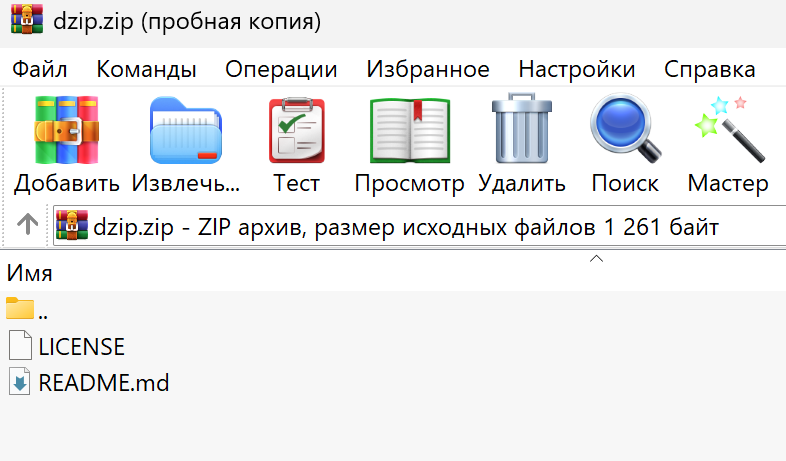
\includegraphics[width=0.6\linewidth]{images/dzip.png}
    \caption{Дешифрованный zip-файл}
    \label{fig:zd}
\end{figure}
